% Source PDF page 610 (printed p. 596), section 11.6 begins here.
\section{含广义不等式的问题}
本节说明怎样将障碍法扩展到含广义不等式的问题。考虑问题
\begin{equation}\begin{aligned}
\text{最小化}\quad&f_0(x)\\
\text{约束为}\quad&f_i(x)\preceq_{K_i}0,\quad i=1,\ldots,m,\\
&Ax=b,
\end{aligned}\tag{11.38}\end{equation}
其中 $f_0:\R^n\to\R$ 为凸函数，$f_i:\R^n\to\R^{k_i}$，$i=1,\ldots,k$，为 $K_i$ 凸函数，$K_i\subseteq\R^{k_i}$ 为正常锥。与第11.1节一样，假设 $f_i$ 二阶连续可微，$A\in\R^{p\times n}$ 且 $\rank A=p$，并假设问题可解。

问题 (11.38) 的 KKT 条件为
\begin{equation}\begin{aligned}
Ax^\star&=b,\\
f_i(x^\star)&\preceq_{K_i}0,\quad i=1,\ldots,m,\\
\lambda_i^\star&\succeq_{K_i^*}0,\quad i=1,\ldots,m,\\
\nabla f_0(x^\star)+\sum_{i=1}^m Df_i(x^\star)^\T\lambda_i^\star+A^\T\nu^\star&=0,\\
(\lambda_i^\star)^\T f_i(x^\star)&=0,\quad i=1,\ldots,m,
\end{aligned}\tag{11.39}\end{equation}
其中 $Df_i(x^\star)\in\R^{k_i\times n}$ 是 $f_i$ 在 $x^\star$ 处的导数。假设问题 (11.38) 严格可行，因此 KKT 条件是 $x^\star$ 最优的充要条件。

该方法的建立与标量约束情形平行。一旦将对数函数推广到一般正常锥上，就可以定义问题 (11.38) 的对数障碍函数。此后的推导与标量情形基本相同，特别是中心路径、障碍法和复杂度分析都非常相似。

% Source PDF page 611 (printed p. 597)
\subsection{对数障碍与中心路径}
\subsubsection*{正常锥的广义对数}
首先，为正常锥 $K\subseteq\R^q$ 定义类似 $\log x$ 的函数。若 $\psi:\R^q\to\R$ 满足以下条件，就称它为 $K$ 的\emph{广义对数}。
\begin{itemize}
\item $\psi$ 为凹、闭、二阶连续可微函数，$\dom\psi=\operatorname{int}K$，且当 $y\in\operatorname{int}K$ 时，$\nabla^2\psi(y)\prec0$。
\item 存在常数 $\theta>0$，使得对所有 $y\succ_K0$ 和 $s>0$，都有
\[
\psi(sy)=\psi(y)+\theta\log s.
\]
换言之，沿锥 $K$ 内任一射线，$\psi$ 的行为都像对数。
\end{itemize}
称常数 $\theta$ 为 $\psi$ 的\emph{次数}，因为 $\exp\psi$ 是 $\theta$ 次齐次函数。注意广义对数只在相差一个加法常数的意义下定义：如果 $\psi$ 是 $K$ 的广义对数，则对 $a\in\R$，$\psi+a$ 也是。普通对数当然是 $\R_+$ 的广义对数。

将使用任意广义对数都满足的以下两个性质。若 $y\succ_K0$，则
\begin{equation}
\nabla\psi(y)\succ_{K^*}0,\tag{11.40}
\end{equation}
这说明 $\psi$ 是 $K$ 递增的（见第3.6.1节），而且
\[
y^\T\nabla\psi(y)=\theta.
\]
第一个性质在习题11.15中证明。第二个性质对 $\psi(sy)=\psi(y)+\theta\log s$ 关于 $s$ 求导即可得到。

\begin{origexample}{11.5}
\emph{非负正交锥。} 函数 $\psi(x)=\sum_{i=1}^n\log x_i$ 是 $K=\R_+^n$ 的广义对数，次数为 $n$。对 $x\succ0$，
\[
\nabla\psi(x)=(1/x_1,\ldots,1/x_n),
\]
因此 $\nabla\psi(x)\succ0$，且 $x^\T\nabla\psi(x)=n$。
\end{origexample}

\begin{origexample}{11.6}
\emph{二阶锥。} 函数
\[
\psi(x)=\log\left(x_{n+1}^2-\sum_{i=1}^n x_i^2\right)
\]
是二阶锥
\[
K=\left\{x\in\R^{n+1}\;\middle|\;\left(\sum_{i=1}^n x_i^2\right)^{1/2}\le x_{n+1}\right\}
\]
% Source PDF page 612 (printed p. 598)
的广义对数，次数为 $2$。$\psi$ 在 $x\in\operatorname{int}K$ 处的梯度为
\[
\frac{\partial\psi(x)}{\partial x_j}=\frac{-2x_j}{x_{n+1}^2-\sum_{i=1}^n x_i^2},\quad j=1,\ldots,n,
\qquad
\frac{\partial\psi(x)}{\partial x_{n+1}}=\frac{2x_{n+1}}{x_{n+1}^2-\sum_{i=1}^n x_i^2}.
\]
容易验证 $\nabla\psi(x)\in\operatorname{int}K^*=\operatorname{int}K$ 和 $x^\T\nabla\psi(x)=2$。
\end{origexample}

\begin{origexample}{11.7}
\emph{半正定锥。} 函数 $\psi(X)=\log\det X$ 是锥 $\mathbf S_+^p$ 的广义对数，次数为 $p$，因为对 $s>0$，
\[
\log\det(sX)=\log\det X+p\log s.
\]
$\psi$ 在 $X\in\mathbf S_{++}^p$ 处的梯度等于
\[
\nabla\psi(X)=X^{-1}.
\]
于是 $\nabla\psi(X)=X^{-1}\succ0$，而 $X$ 与 $\nabla\psi(X)$ 的内积等于 $\tr(XX^{-1})=p$。
\end{origexample}

\subsubsection*{广义不等式的对数障碍函数}
回到问题 (11.38)，设 $\psi_1,\ldots,\psi_m$ 分别为锥 $K_1,\ldots,K_m$ 的广义对数，次数为 $\theta_1,\ldots,\theta_m$。定义问题 (11.38) 的对数障碍函数为
\[
\phi(x)=-\sum_{i=1}^m\psi_i(-f_i(x)),\qquad
\dom\phi=\{x\mid f_i(x)\prec_{K_i}0,\ i=1,\ldots,m\}.
\]
$\phi$ 的凸性来自 $\psi_i$ 的 $K_i$ 递增性以及 $f_i$ 的 $K_i$ 凸性，见第3.6.2节的复合规则。

\subsubsection*{中心路径}
下一步定义问题 (11.38) 的中心路径。对 $t\ge0$，将中心点 $x^\star(t)$ 定义为 $tf_0+\phi$ 在 $Ax=b$ 约束下的最小化点，即问题
\[
\begin{aligned}
\text{最小化}\quad&tf_0(x)-\sum_{i=1}^m\psi_i(-f_i(x))\\
\text{约束为}\quad&Ax=b
\end{aligned}
\]
的解，假设最小化点存在且唯一。中心点由最优性条件
\begin{equation}\begin{aligned}
t\nabla f_0(x)+\nabla\phi(x)+A^\T\nu
&=t\nabla f_0(x)+\sum_{i=1}^m Df_i(x)^\T\nabla\psi_i(-f_i(x))+A^\T\nu\\
&=0
\end{aligned}\tag{11.41}\end{equation}
刻画，其中某个 $\nu\in\R^p$ 存在，$Df_i(x)$ 是 $f_i$ 在 $x$ 处的导数。

% Source PDF page 613 (printed p. 599)
\subsubsection*{中心路径上的对偶点}
与标量情形一样，中心路径上的点给出问题 (11.38) 的对偶可行点。对 $i=1,\ldots,m$，定义
\begin{equation}
\lambda_i^\star(t)=\frac1t\nabla\psi_i(-f_i(x^\star(t))),\tag{11.42}
\end{equation}
令 $\nu^\star(t)=\nu/t$，其中 $\nu$ 是 (11.41) 中的最优对偶变量。下面证明 $\lambda_1^\star(t),\ldots,\lambda_m^\star(t)$ 连同 $\nu^\star(t)$，对原问题 (11.38) 对偶可行。

首先，由广义对数的单调性 (11.40)，$\lambda_i^\star(t)\succ_{K_i^*}0$。其次，由 (11.41) 可知，拉格朗日函数
\[
L(x,\lambda^\star(t),\nu^\star(t))=f_0(x)+\sum_{i=1}^m\lambda_i^\star(t)^\T f_i(x)
+\nu^\star(t)^\T(Ax-b)
\]
在 $x=x^\star(t)$ 处取得最小值。因此，对偶函数 $g$ 在 $(\lambda^\star(t),\nu^\star(t))$ 处的值为
\begin{align*}
g(\lambda^\star(t),\nu^\star(t))
&=f_0(x^\star(t))+\sum_{i=1}^m\lambda_i^\star(t)^\T f_i(x^\star(t))
+\nu^\star(t)^\T(Ax^\star(t)-b)\\
&=f_0(x^\star(t))+(1/t)\sum_{i=1}^m\nabla\psi_i(-f_i(x^\star(t)))^\T f_i(x^\star(t))\\
&=f_0(x^\star(t))-(1/t)\sum_{i=1}^m\theta_i,
\end{align*}
其中 $\theta_i$ 为 $\psi_i$ 的次数。最后一行使用了 $y\succ_{K_i}0$ 时 $y^\T\nabla\psi_i(y)=\theta_i$，因此
\begin{equation}
\lambda_i^\star(t)^\T f_i(x^\star(t))=-\theta_i/t,\quad i=1,\ldots,m.\tag{11.43}
\end{equation}
于是定义
\[
\bar\theta=\sum_{i=1}^m\theta_i,
\]
则原始可行点 $x^\star(t)$ 与对偶可行点 $(\lambda^\star(t),\nu^\star(t))$ 的对偶间隙为 $\bar\theta/t$。这与标量情形相同，只不过不等式数 $m$ 被各锥广义对数次数之和 $\bar\theta$ 替代。

\begin{origexample}{11.8}
\emph{二阶锥规划。} 考虑变量为 $x\in\R^n$ 的 SOCP：
\begin{equation}\begin{aligned}
\text{最小化}\quad&f^\T x\\
\text{约束为}\quad&\norm{A_i x+b_i}_2\le c_i^\T x+d_i,\quad i=1,\ldots,m,
\end{aligned}\tag{11.44}\end{equation}
其中 $A_i\in\R^{n_i\times n}$。正如例11.6所示，函数
\[
\psi(y)=\log\left(y_{p+1}^2-\sum_{i=1}^p y_i^2\right)
\]
% Source PDF page 614 (printed p. 600)
是 $\R^{p+1}$ 中二阶锥的广义对数，次数为 $2$。对应于 (11.44) 的对数障碍函数为
\begin{equation}
\phi(x)=-\sum_{i=1}^m\log\bigl((c_i^\T x+d_i)^2-\norm{A_i x+b_i}_2^2\bigr),\tag{11.45}
\end{equation}
其定义域为 $\dom\phi=\{x\mid\norm{A_i x+b_i}_2<c_i^\T x+d_i,\ i=1,\ldots,m\}$。中心路径上的最优性条件为 $tf+\nabla\phi(x^\star(t))=0$，其中
\[
\nabla\phi(x)=-2\sum_{i=1}^m
\frac{(c_i^\T x+d_i)c_i-A_i^\T(A_i x+b_i)}{(c_i^\T x+d_i)^2-\norm{A_i x+b_i}_2^2}.
\]
因此，点
\[
z_i^\star(t)=\frac{-2}{t\alpha_i}(A_i x^\star(t)+b_i),\qquad
w_i^\star(t)=\frac2{t\alpha_i}(c_i^\T x^\star(t)+d_i),\quad i=1,\ldots,m,
\]
其中 $\alpha_i=(c_i^\T x^\star(t)+d_i)^2-\norm{A_i x^\star(t)+b_i}_2^2$，对对偶问题
\[
\begin{aligned}
\text{最大化}\quad&-\sum_{i=1}^m(b_i^\T z_i+d_i w_i)\\
\text{约束为}\quad&\sum_{i=1}^m(A_i^\T z_i+c_i w_i)=f,\\
&\norm{z_i}_2\le w_i,\quad i=1,\ldots,m
\end{aligned}
\]
严格可行。$x^\star(t)$ 与 $(z^\star(t),w^\star(t))$ 对应的对偶间隙为
\[
\sum_{i=1}^m\bigl((A_i x^\star(t)+b_i)^\T z_i^\star(t)
+(c_i^\T x^\star(t)+d_i)w_i^\star(t)\bigr)=\frac{2m}{t},
\]
与一般公式 $\bar\theta/t$ 一致，因为 $\theta_i=2$。
\end{origexample}

\begin{origexample}{11.9}
\emph{不等式形式的半定规划。} 考虑变量为 $x\in\R^n$ 的 SDP
\[
\begin{aligned}\text{最小化}\quad&c^\T x\\\text{约束为}\quad&F(x)=x_1F_1+\cdots+x_nF_n+G\preceq0,\end{aligned}
\]
其中 $G,F_1,\ldots,F_n\in\mathbf S^p$。其对偶问题为
\[
\begin{aligned}\text{最大化}\quad&\tr(GZ)\\\text{约束为}\quad&\tr(F_iZ)+c_i=0,\quad i=1,\ldots,n,\\&Z\succeq0.\end{aligned}
\]
使用半正定锥 $\mathbf S_+^p$ 的广义对数 $\log\det X$，得到原始问题的障碍函数
\[
\phi(x)=\log\det(-F(x)^{-1}),\qquad\dom\phi=\{x\mid F(x)\prec0\}.
\]
对严格可行的 $x$，$\phi$ 的梯度为
\[
\frac{\partial\phi(x)}{\partial x_i}=\tr(-F(x)^{-1}F_i),\quad i=1,\ldots,n,
\]
由此得到刻画中心点的最优性条件
\[
tc_i+\tr(-F(x^\star(t))^{-1}F_i)=0,\quad i=1,\ldots,n.
\]
因此矩阵
\[
Z^\star(t)=\frac1t(-F(x^\star(t)))^{-1}
\]
严格对偶可行，$x^\star(t)$ 与 $Z^\star(t)$ 对应的对偶间隙为 $p/t$。
\end{origexample}

% Source PDF page 615 (printed p. 601)
\subsection{障碍法}
我们已经看到，中心路径的关键性质可以推广到含广义不等式的问题。
\begin{itemize}
\item 计算中心路径上的一个点，就是在等式约束下最小化一个二阶可微凸函数，可用牛顿法完成。
\item 对中心点 $x^\star(t)$，可以构造一个对偶可行点 $(\lambda^\star(t),\nu^\star(t))$，对应对偶间隙为 $\bar\theta/t$。特别地，$x^\star(t)$ 的次优程度不超过 $\bar\theta/t$。
\end{itemize}
这意味着，可以完全按第11.3节的方法对问题 (11.38) 应用障碍法。从 $x^\star(t^{(0)})$ 出发，计算对偶间隙为 $\epsilon$ 的中心点所需的外迭代或中心化次数为
\[
\left\lceil\frac{\log(\bar\theta/(t^{(0)}\epsilon))}{\log\mu}\right\rceil,
\]
再加一次初始中心化。这个结果与标量情形的唯一区别，是以 $\bar\theta$ 代替 $m$。

\subsubsection*{第一阶段与可行性问题}
第11.4节的第一阶段方法很容易推广到含广义不等式的问题。对 $i=1,\ldots,m$，设给定 $K_i$ 正向量 $e_i\succ_{K_i}0$。为确定等式与广义不等式组
\[
f_1(x)\preceq_{K_1}0,\quad\ldots,\quad f_L(x)\preceq_{K_m}0,\qquad Ax=b
\]
的可行性，求解问题
\[
\begin{aligned}\text{最小化}\quad&s\\\text{约束为}\quad&f_i(x)\preceq_{K_i}se_i,\quad i=1,\ldots,m,\\&Ax=b,\end{aligned}
\]
变量为 $x$ 与 $s\in\R$。最优值 $\bar p^\star$ 决定该等式与广义不等式组的可行性，与普通不等式的情形完全相同。$\bar p^\star$ 为正时，任意目标为正的对偶可行点都给出一个择一系统的解，证明原等式与广义不等式组不可行，见第270页。

\subsection{例子}
\subsubsection*{小型 SOCP}
求解 SOCP
\[
\begin{aligned}\text{最小化}\quad&f^\T x\\\text{约束为}\quad&\norm{A_i x+b_i}_2\le c_i^\T x+d_i,\quad i=1,\ldots,m,\end{aligned}
\]
% Source PDF page 616 (printed p. 602)
其中 $x\in\R^{50}$、$m=50$、$A_i\in\R^{5\times50}$。随机生成实例，使其严格原始可行、严格对偶可行，最优值 $p^\star=1$。从中心路径上的点 $x^{(0)}$ 出发，对偶间隙为 $100$。

\begin{figure}[htbp]\centering
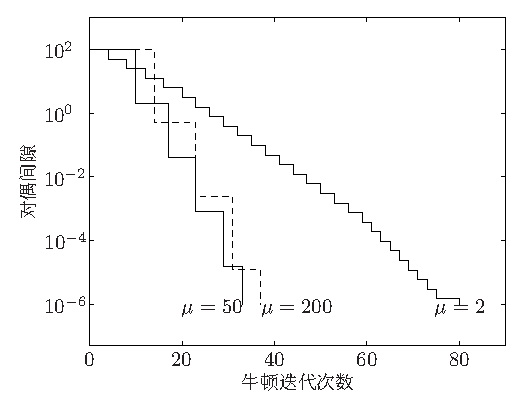
\includegraphics[width=.65\textwidth]{figures/ch11-15.pdf}
\caption*{图11.15 SOCP 的障碍法求解进展，展示对偶间隙与累计牛顿步数的关系。}
\end{figure}
用障碍法求解该问题，障碍函数为
\[
\phi(x)=-\sum_{i=1}^m\log\bigl((c_i^\T x+d_i)^2-\norm{A_i x+b_i}_2^2\bigr).
\]
中心化问题用牛顿法求解，算法参数与第11.3.2节例子相同：回溯参数 $\alpha=0.01$、$\beta=0.5$，停止准则为 $\lambda(x)^2/2\le10^{-5}$。

图11.15给出对偶间隙随累计牛顿步数的变化。它与线性规划和几何规划的图11.4与图11.6非常相似：每次中心化所需牛顿步数近似不变，因此对偶间隙近似线性收敛。对这个例子，只要 $\mu$ 至少约为 $10$，其选择对总牛顿步数也影响很小。与线性规划、几何规划的例子一样，$\mu$ 取 $10$ 至 $100$ 较合理，此时总牛顿步数约为 $30$，见图11.16。

\subsubsection*{小型 SDP}
下一个例子是 SDP
\begin{equation}\begin{aligned}\text{最小化}\quad&c^\T x\\\text{约束为}\quad&\sum_{i=1}^n x_iF_i+G\preceq0,
\end{aligned}\tag{11.46}\end{equation}
% Source PDF page 617 (printed p. 603)
变量为 $x\in\R^{100}$，且 $F_i\in\mathbf S^{100}$、$G\in\mathbf S^{100}$。随机生成实例，使其严格原始可行、严格对偶可行，且 $p^\star=1$。初始点位于中心路径上，对偶间隙为 $100$。

\begin{figure}[htbp]\centering
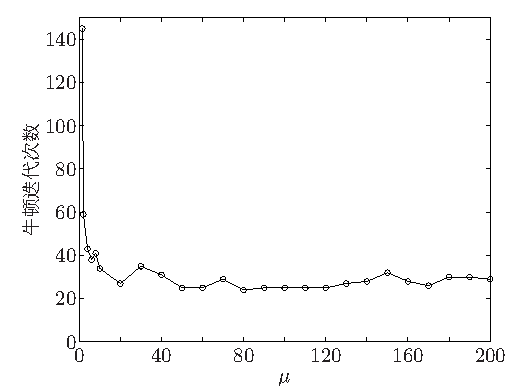
\includegraphics[width=.65\textwidth]{figures/ch11-16.pdf}
\caption*{图11.16 小型 SOCP 中参数 $\mu$ 的选择权衡。纵轴为将对偶间隙从 $100$ 降低到 $10^{-3}$ 所需的总牛顿步数，横轴为 $\mu$。}
\end{figure}
应用障碍法，对数障碍函数为
\[
\phi(x)=-\log\det\left(-\sum_{i=1}^n x_iF_i-G\right).
\]
图11.17展示了三个 $\mu$ 值下的障碍法进展。注意它与线性规划、几何规划、二阶锥规划的图11.4、图11.6和图11.15相似。与其他例子一样，只要 $\mu$ 不太小，它对效率的影响就很小。图11.18给出将对偶间隙缩小 $10^5$ 倍所需牛顿步数与 $\mu$ 的关系。

\subsubsection*{一族 SDP}
本节考察障碍法性能随问题维数的变化。考虑如下形式的一族 SDP：
\begin{equation}\begin{aligned}
\text{最小化}\quad&\one^\T x\\\text{约束为}\quad&A+\diag(x)\succeq0,
\end{aligned}\tag{11.47}\end{equation}
变量为 $x\in\R^n$，参数为 $A\in\mathbf S^n$。矩阵 $A$ 按如下方式生成：$i\ge j$ 时，从相互独立的 $\mathcal N(0,1)$ 分布生成 $A_{ij}$；$i<j$ 时取 $A_{ij}=A_{ji}$，使 $A\in\mathbf S^n$。再缩放 $A$，使其谱范数为 $1$。

% Source PDF page 618 (printed p. 604)
\begin{figure}[htbp]\centering
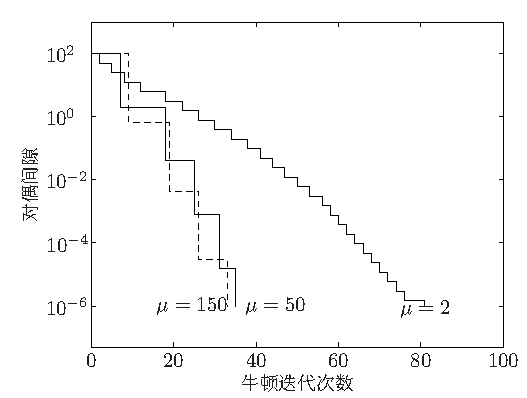
\includegraphics[width=.65\textwidth]{figures/ch11-17.pdf}
\caption*{图11.17 小型 SDP 的障碍法进展：对偶间隙与累计牛顿步数的关系。三条曲线分别对应 $\mu=2,50,150$。}
\end{figure}
\begin{figure}[htbp]\centering
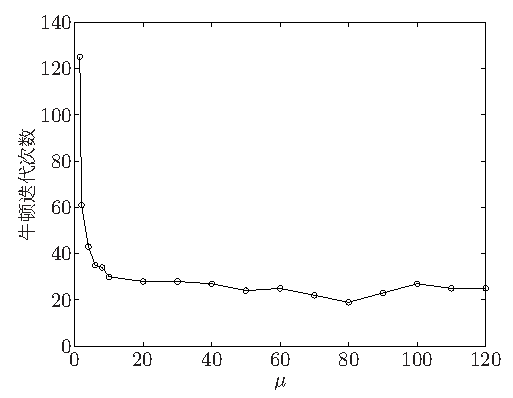
\includegraphics[width=.65\textwidth]{figures/ch11-18.pdf}
\caption*{图11.18 小型 SDP 中参数 $\mu$ 的选择权衡。纵轴为将对偶间隙从 $100$ 降低到 $10^{-3}$ 所需的总牛顿步数，横轴为 $\mu$。}
\end{figure}

% Source PDF page 619 (printed p. 605)
\begin{figure}[htbp]\centering
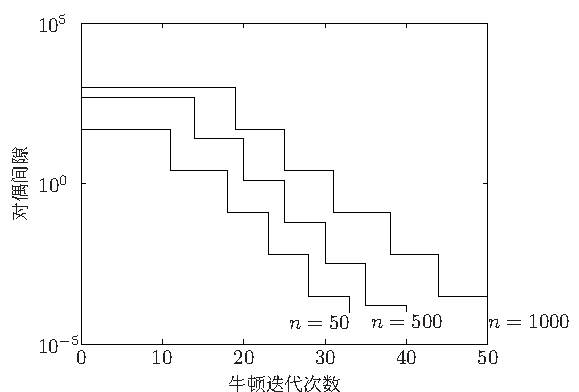
\includegraphics[width=.7\textwidth]{figures/ch11-19.pdf}
\caption*{图11.19 三个不同维数的随机 SDP (11.47) 的障碍法进展。图中展示对偶间隙与累计牛顿步数的关系，每个问题的变量数为 $n$。}
\end{figure}
算法参数取 $\mu=20$，中心化参数与上面各例相同：回溯参数 $\alpha=0.01$、$\beta=0.5$，停止准则 $\lambda(x)^2/2\le10^{-5}$。初始点位于中心路径上，$t^{(0)}=1$，即间隙为 $n$。当初始对偶间隙缩小 $8000$ 倍，即完成三次外迭代时，算法终止。

图11.19给出维数 $n=50$、$n=500$、$n=1000$ 的三个实例中，对偶间隙与迭代次数的关系。曲线与前面各图非常相似，也与 LP 的曲线非常相似。

为考察问题规模对所需牛顿步数的影响，对 $n=10$ 至 $n=1000$ 之间的 $20$ 个值，每个值生成 $100$ 个问题实例。用障碍法求解这 $2000$ 个问题，记录所需牛顿步数。图11.20汇总了每个 $n$ 下牛顿步数的均值与标准差。该图与 LP 的图11.8很相似。特别地，问题维数扩大 $100$ 倍时，所需牛顿步数增长很慢，仅从约 $20$ 次增加到 $26$ 次。

\subsection{基于自协调性的复杂度分析}
本节将第11.5节普通不等式问题的障碍法复杂度分析，推广到广义不等式问题。我们已经看到，外迭代次数为
\[
\left\lceil\frac{\log(\bar\theta/(t^{(0)}\epsilon))}{\log\mu}\right\rceil,
\]
% Source PDF page 620 (printed p. 606)
再加一次初始中心化。剩下需要界定每次中心化的牛顿步数，这将使用自协调函数的牛顿法复杂度理论。为简便起见，不计初始中心化的成本。

\begin{figure}[htbp]\centering
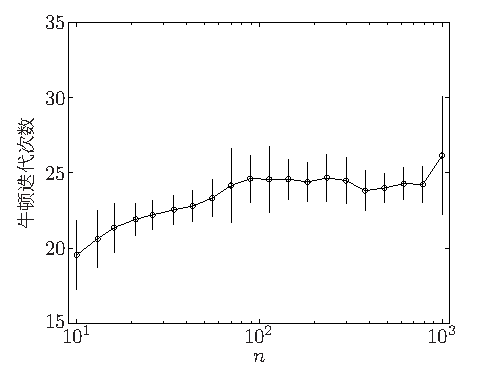
\includegraphics[width=.6\textwidth]{figures/ch11-20.pdf}
\caption*{图11.20 对问题规模 $n$ 的 $20$ 个值，每个值求解 $100$ 个随机 SDP (11.47) 所需的平均牛顿步数。误差棒给出每个 $n$ 下围绕均值的标准差。问题维数在 $100:1$ 的范围内变化时，平均牛顿步数的增长很小。}
\end{figure}
与第11.5节作相同假设：对所有 $t\ge t^{(0)}$，函数 $tf_0+\phi$ 为自协调闭函数，且 (11.38) 的下水平集有界。

\begin{origexample}{11.10}
\emph{二阶锥规划。} 函数
\[
-\psi(x)=-\log\left(x_{p+1}^2-\sum_{i=1}^p x_i^2\right)
\]
自协调（见例9.8），因此 SOCP (11.44) 的对数障碍函数 (11.45) 满足闭性和自协调性假设。
\end{origexample}

\begin{origexample}{11.11}
\emph{半定规划。} 以 $\log\det X$ 为半正定锥的广义对数时，一般半定规划满足自协调性假设。例如，标准形式 SDP
\[
\begin{aligned}\text{最小化}\quad&\tr(CX)\\\text{约束为}\quad&\tr(A_iX)=b_i,\quad i=1,\ldots,p,\\&X\succeq0,\end{aligned}
\]
变量为 $X\in\mathbf S^n$，对任意 $t^{(0)}\ge0$，函数 $t^{(0)}\tr(CX)-\log\det X$ 都是自协调闭函数。
\end{origexample}

% Source PDF page 621 (printed p. 607)
将看到，与标量情形完全一样，有
\begin{equation}\begin{aligned}
\mu t f_0(x^\star(t))+\phi(x^\star(t))-\mu t f_0(x^\star(\mu t))-\phi(x^\star(\mu t))
\le\bar\theta(\mu-1-\log\mu).
\end{aligned}\tag{11.48}\end{equation}
因此，自协调性与下水平集有界条件成立时，每次中心化所需的牛顿步数不超过
\[
\frac{\bar\theta(\mu-1-\log\mu)}\gamma+c,
\]
与普通不等式问题的障碍法完全相同。一旦建立基本界 (11.48)，广义不等式问题的复杂度分析就与普通不等式问题一致，唯一区别是以各锥次数之和 $\bar\theta$ 代替不等式数。

\subsubsection*{对偶锥的广义对数}
将用共轭函数证明界 (11.48)。设 $\psi$ 是正常锥 $K$ 的广义对数，次数为 $\theta$。凸函数 $-\psi$ 的共轭为
\[
(-\psi)^*(v)=\sup_u\bigl(v^\T u+\psi(u)\bigr).
\]
该函数为凸函数，定义域为 $-K^*=\{v\mid v\prec_{K^*}0\}$。定义 $\bar\psi$ 为
\begin{equation}
\bar\psi(v)=-(-\psi)^*(-v)=\inf_u\bigl(v^\T u-\psi(u)\bigr),\qquad
\dom\bar\psi=\operatorname{int}K^*.\tag{11.49}
\end{equation}
函数 $\bar\psi$ 为凹函数，实际上它也是对偶锥 $K^*$ 的广义对数，参数同样为 $\theta$，见习题11.17。称 $\bar\psi$ 为与广义对数 $\psi$ 对应的\emph{对偶对数}。

由 (11.49) 得到不等式
\begin{equation}
\bar\psi(v)+\psi(u)\le u^\T v,\tag{11.50}
\end{equation}
它对任意 $u\succ_K0$、$v\succ_{K^*}0$ 成立，等号成立当且仅当 $\nabla\psi(u)=v$，或等价地 $\nabla\bar\psi(v)=u$。（这只是凹函数版本 Young 不等式的一个变体。）

\begin{origexample}{11.12}
\emph{二阶锥。} 二阶锥的广义对数为
\[
\psi(x)=\log\left(x_{p+1}^2-\sum_{i=1}^p x_i^2\right),\qquad
\dom\psi=\left\{x\in\R^{p+1}\;\middle|\;x_{p+1}>\left(\sum_{i=1}^p x_i^2\right)^{1/2}\right\}.
\]
对应的对偶对数为
\[
\bar\psi(y)=\log\left(y_{p+1}^2-\sum_{i=1}^p y_i^2\right)+2-\log4,
\]
定义域为 $\dom\bar\psi=\{y\in\R^{p+1}\mid y_{p+1}>(\sum_{i=1}^p y_i^2)^{1/2}\}$，见习题3.36。除一个常数外，它与二阶锥原来的广义对数相同。
\end{origexample}

% Source PDF page 622 (printed p. 608)
\begin{origexample}{11.13}
\emph{半正定锥。} 与 $\psi(X)=\log\det X$、$\dom\psi=\mathbf S_{++}^p$ 对应的对偶对数为
\[
\bar\psi(Y)=\log\det Y+p,
\]
定义域为 $\dom\psi^*=\mathbf S_{++}^p$，见例3.23。同样，除一个常数外，它是同一个广义对数。
\end{origexample}

\subsubsection*{基本界的推导}
为简化记号，将 $x^\star(t)$ 记为 $x$，$x^\star(\mu t)$ 记为 $x^+$，$\lambda_i^\star(t)$ 记为 $\lambda_i$，$\nu^\star(t)$ 记为 $\nu$。由 (11.42) 中的 $t\lambda_i=\nabla\psi_i(-f_i(x))$ 以及性质 (11.43)，得到
\begin{equation}
\psi_i(-f_i(x))+\bar\psi_i(t\lambda_i)=-t\lambda_i^\T f_i(x)=\theta_i,\tag{11.51}
\end{equation}
即 (11.50) 对 $u=-f_i(x)$、$v=t\lambda_i$ 取等号。将同一不等式应用于 $u=-f_i(x^+)$、$v=\mu t\lambda_i$，得到
\[
\psi_i(-f_i(x^+))+\bar\psi_i(\mu t\lambda_i)\le-\mu t\lambda_i^\T f_i(x^+).
\]
利用 $\bar\psi_i$ 的对数齐次性，变为
\[
\psi_i(-f_i(x^+))+\bar\psi_i(t\lambda_i)+\theta_i\log\mu\le-\mu t\lambda_i^\T f_i(x^+).
\]
从这个不等式中减去等式 (11.51)，得到
\[
-\psi_i(-f_i(x))+\psi_i(-f_i(x^+))+\theta_i\log\mu
\le-\theta_i-\mu t\lambda_i^\T f_i(x^+).
\]
对 $i$ 求和，得到
\begin{equation}
\phi(x)-\phi(x^+)+\bar\theta\log\mu\le-\bar\theta-\mu t\sum_{i=1}^m\lambda_i^\T f_i(x^+).\tag{11.52}
\end{equation}
另由对偶函数的定义，
\begin{align*}
f_0(x)-\bar\theta/t&=g(\lambda,\nu)\\
&\le f_0(x^+)+\sum_{i=1}^m\lambda_i^\T f_i(x^+)+\nu^\T(Ax^+-b)\\
&=f_0(x^+)+\sum_{i=1}^m\lambda_i^\T f_i(x^+).
\end{align*}
将该不等式乘以 $\mu t$，再与 (11.52) 相加，得到
\[
\phi(x)-\phi(x^+)+\bar\theta\log\mu+\mu t f_0(x)-\mu\bar\theta
\le\mu t f_0(x^+)-\bar\theta.
\]
整理后为
\[
\mu t f_0(x)+\phi(x)-\mu t f_0(x^+)-\phi(x^+)\le\bar\theta(\mu-1-\log\mu),
\]
这就是所需不等式 (11.48)。
